% \VignetteIndexEntry{doRedis Manual}
% \VignetteDepends{doRedis}
% \VignettePackage{doRedis}
\documentclass[12pt]{article}
\usepackage{amsmath}
%\usepackage{lmodern}
\usepackage[pdftex]{graphicx}
\usepackage{color}
\usepackage{xspace}
\usepackage{fancyvrb}
\usepackage{fancyhdr}
\usepackage[
     colorlinks=true,
     linkcolor=blue,
     citecolor=blue,
     urlcolor=blue]
     {hyperref}
\usepackage{lscape}
\usepackage{Sweave}
\usepackage{tabularx}
\usepackage{listings,relsize}
\usepackage{upquote}
\lstloadlanguages{R}
\lstset{frame=none, basicstyle=\footnotesize\ttfamily, commentstyle=\rmfamily\small, showstringspaces=false, literate={'}{{$^{\prime}$}}{1} {~}{{$\sim$}}1,escapeinside={(*}{*)}}   % for (*\ref{ }*) inside lstlistings (S code)
\usepackage{caption}
\DeclareCaptionFont{white}{\color{white}}
\DeclareCaptionFormat{listing}{\colorbox{gray}{\parbox{\textwidth}{#1#2#3}}}
\captionsetup[lstlisting]{format=listing,labelfont=white,textfont=white,margin=0pt}


%%%%%%%%%%%%%%%%%%%%%%%%%%%%%%%%%%%%%%%%%%%%%%%%%%%%%%%%%%%%%%%%%%

% define new colors for use
\definecolor{gray}{rgb}{0.4,0.4,0.4}
\definecolor{darkgreen}{rgb}{0,0.6,0}
\definecolor{darkred}{rgb}{0.6,0.0,0}
\definecolor{lightbrown}{rgb}{1,0.9,0.8}
\definecolor{brown}{rgb}{0.6,0.3,0.3}
\definecolor{darkblue}{rgb}{0,0,0.8}
\definecolor{darkmagenta}{rgb}{0.5,0,0.5}

%%%%%%%%%%%%%%%%%%%%%%%%%%%%%%%%%%%%%%%%%%%%%%%%%%%%%%%%%%%%%%%%%%

\newcommand{\bld}[1]{\mbox{\boldmath $#1$}}
\newcommand{\shell}[1]{\mbox{$#1$}}
\renewcommand{\vec}[1]{\mbox{\bf {#1}}}
\newcommand{\ReallySmallSpacing}{\renewcommand{\baselinestretch}{.6}\Large\normalsize}
\newcommand{\SmallSpacing}{\renewcommand{\baselinestretch}{1.1}\Large\normalsize}
\def\tm{\leavevmode\hbox{$\rm {}^{TM}$}}

\newenvironment{mitemize}{
\begin{itemize}
  \setlength{\itemsep}{1pt}
  \setlength{\parskip}{0pt}
  \setlength{\parsep}{0pt}
}{\end{itemize}}


\setlength{\oddsidemargin}{-.25 truein}
\setlength{\evensidemargin}{0truein}
\setlength{\topmargin}{-0.2truein}
\setlength{\textwidth}{7 truein}
\setlength{\textheight}{8.5 truein}
\setlength{\parindent}{0.20truein}
\setlength{\parskip}{0.10truein}

%%%%%%%%%%%%%%%%%%%%%%%%%%%%%%%%%%%%%%%%%%%%%%%%%%%%%%%%%%%%%%%%%%
\pagestyle{fancy}
\lhead{}
\chead{The {\tt doRedis} Package}
\rhead{}
\lfoot{}
\cfoot{}
\rfoot{\thepage}
\renewcommand{\headrulewidth}{1pt}
\renewcommand{\footrulewidth}{1pt}
%%%%%%%%%%%%%%%%%%%%%%%%%%%%%%%%%%%%%%%%%%%%%%%%%%%%%%%%%%%%%%%%%%
\title{Introduction to the {\tt doRedis} Package}
\author{Bryan W. Lewis \\ 
blewis@illposed.net}

\begin{document}

\maketitle

\thispagestyle{empty}

\section{Introduction}

The {\tt doRedis} package provides a parallel back end for {\tt foreach} using
Redis and the corresponding {\tt rredis} package. It lets users easily run
parallel jobs across multiple R sessions.

Steve Weston's {\tt foreach} package is a remarkable parallel computing
framework for the R language. Similarly to lapply-like functions, foreach maps
functions to data and aggregates results. Even better, foreach lets you do this
in parallel across multiple CPU cores and computers.  And even better yet,
foreach abstracts the parallel computing details away into modular back end
code. Code written using foreach works sequentially in the absence of a
parallel back end, and works uniformly across different back ends, allowing
programmers to write code independently of specific parallel computing
implementations. The {\tt foreach} package has many other wonderful features
outlined in its package documentation.

Redis is a fast, persistent, networked database with many innovative features,
among them a blocking queue-like data structure (Redis ``lists''). This feature
makes Redis useful as a lightweight back end for parallel computing.  The
{\tt rredis} package provides a native R interface to Redis used by
{\tt doRedis}.

\subsection{Why doRedis?}

Why write a {\tt doRedis} package? After all, the {\tt foreach} package already
has available many parallel back end packages, including {\tt doMC}, 
{\tt doSNOW} and {\tt doMPI}.

The key differentiating features of {\tt doRedis} are elasticity and fault-tolerance,
and portability across operating system platforms. The {\tt doRedis} package is
well-suited to small to medium-sized parallel computing jobs, especially across
ad hoc collections of computing resources.

\begin{itemize}
%\renewcommand{\labelitemi}{{\bf{--}}}

\item {\tt doRedis} allows for dynamic pools of workers. New workers may be
added at any time, even in the middle of running computations.  This feature is
geared for modern cloud computing environments.  Users can make an economic
decision to ``turn on'' more computing resources at any time in order to
accelerate running computations. Similarly, modern cluster resource allocation
systems can dynamically schedule R workers as cluster resources become
available.

\item {\tt doRedis} computations are partially fault tolerant. Failure of
back-end worker R processes (for example due to a machine crash or simply
scaling back elastic resources) are automatically detected and the affected
tasks are automatically re-submitted.

\item {\tt doRedis} makes it particularly easy to run parallel jobs across
different operating systems. It works equally well on GNU/Linux, Mac OS X, and
Windows systems, and should work well on most POSIX systems.  Back end parallel
R worker processes are effectively anonymous--they may run anywhere as long as
all the R package dependencies required by the task at hand are available.

\item Like all {\tt foreach} parallel back-ends, intermediate results may be
aggregated incrementally, significantly reducing required memory overhead for
problems that return large data.

\end{itemize}





\section{Obtaining and Configuring the Redis server}\label{install}

Redis is an extremely popular open source networked key/value database, and
operating system-specific packages are available for all major operating
systems, including Windows.

For more information see:
\htmladdnormallink{http://redis.io/download}{http://redis.io/download}.

The Redis server is completely configured by the file \verb+redis.conf+.  It's
important to make sure that the \verb+timeout+ setting is set to \verb+0+ in
the \verb+redis.conf+ file when using {\tt doRedis}.  You may wish to peruse
the rest of the configuration file and experiment with the other server
settings as well.


\section{doRedis Examples}

Let's start by exploring the operation of some {\tt doRedis} features through a
few examples.  Unless otherwise noted, we assume that Redis is installed and
running on the local computer (``localhost'').

\subsection{A Really Simple Example}

The simple example below is one version of a Monte Carlo
approximation of $\pi$. Variations on this example are often used to
illustrate parallel programming ideas. 
\begin{lstlisting}[float=ht,caption=Monte Carlo Example]
> library("doRedis")
> registerDoRedis("jobs")
> startLocalWorkers(n=2, queue="jobs")
> foreach(icount(10),.combine=sum,
+          .multicombine=TRUE,.inorder=FALSE) %dopar%
+          4*sum((runif(1000000)^2 + runif(1000000)^2)<1)/10000000
[1] 3.144212
removeQueue("jobs")
\end{lstlisting}
\begin{center}
\resizebox{0.6\textwidth}{!}{\rotatebox{0}{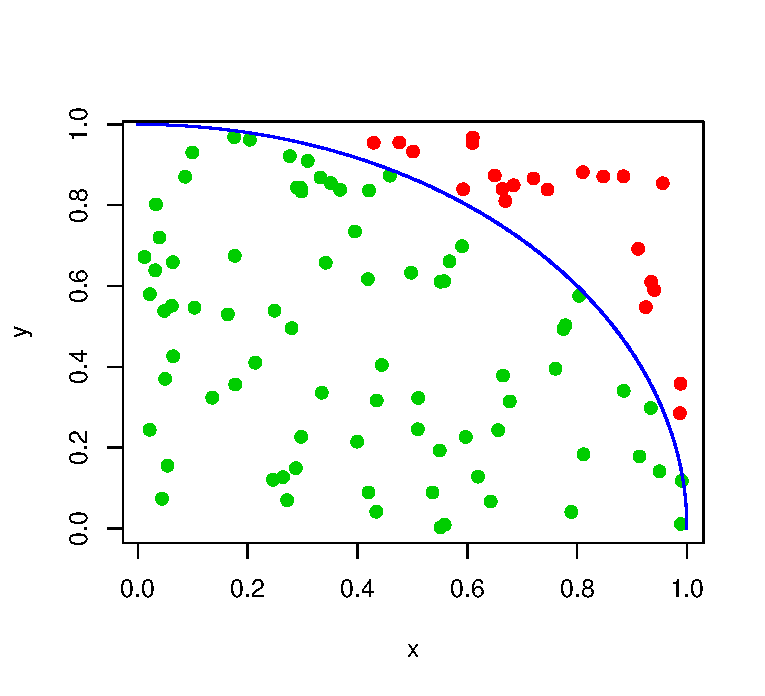
\includegraphics{circle}}}
\end{center}
The figure illustrates how the method works. We randomly choose points in the
unit square. The ratio of points that lie inside the arc of the unit circle
(green) to the total number of points provides an approximation of the area of
$1/4$ the area of the unit circle--that is, an approximation of $\pi/4$.  Each
one of the 10 iterations (``tasks'' in \verb+doRedis+) of the loop computes a
scaled approximation  of $\pi$ using 1,000,000 such points.  We then sum up
each of the 10 results to get an approximation of $\pi$ using all 10,000,000
points.

The {\tt doRedis} package uses the idea of a ``work queue'' to dole out jobs
to available resources. Each {\tt doRedis} \emph{job} is composed of a set
of one or more \emph{tasks}. Worker R processes listen on the work queue
for new jobs. The line

\noindent \verb+registerDoRedis("jobs")+

\noindent registers the {\tt doRedis} back end with {\tt foreach} using the
user-specified work queue name ``jobs'' (you are free to use any name you wish
for the work queue). R can issue work to a work queue even if there aren't
any workers yet.

The next line:

\noindent \verb+startLocalWorkers(n=2, queue="jobs")+

\noindent starts up two worker R sessions on the local computer, both listening
for work on the queue named ``jobs.'' The worker sessions don't display any 
output by default. The {\tt startLocalWorkers} function can instruct the
workers to log messages to output files or stdout if desired.

You can verify that workers are in fact waiting for work with:

\noindent \verb+getDoParWorkers()+

\noindent which should return 2, for the two workers we just started. Note that
the number of workers may change over time (unlike most other parallel back
ends for {\tt foreach}). The {\tt getDoParWorkers} function returns the current
number of workers in the pool, but the number returned should only be
considered to be an estimate of the actual number of available workers.

The next lines actually run the Monte Carlo code:

\noindent \verb+foreach(icount(10),.combine=sum,.multicombine=TRUE,.inorder=FALSE) %dopar%+
\\
$\phantom{xxxxxx}$\verb_4*sum((runif(1000000)^2 + runif(1000000)^2)<1)/10000000_

\noindent
This parallel loop consists of 10 iterations (tasks in this example) using the 
{\tt icount} iterator function.
We specify that the results from each task should be passed to
the {\tt sum} function with {\tt .combine=sum}.  Setting the {\tt
.multicombine} option to {\tt TRUE} tells {\tt foreach} that the {\tt .combine}
function accepts an arbitrary number of function arguments (some aggregation
functions only work on two arguments). The {\tt .inorder=FALSE} option tells
foreach that results may be passed to the {\tt .combine} function as they 
arrive, in any order. The {\tt \%dopar\%} operator instructs
{\tt foreach} to use the {\tt doRedis} back end that we previously registered
to place each task in the work queue.  Finally, each iteration runs the scaled
estimation of $\pi$ using 1,000,000 points.

\subsection{Fault tolerance}

Parallel computations managed by {\tt doRedis} tolerate failures among the back
end worker R processes. Examples of failures include crashed back end R
sessions, operating system crash or reboot, power outages, or simply dialing
down elastic workers by turning them off. When a failure is detected, affected tasks are
automatically re-submitted to the work queue. The option {\tt ftinterval}
controls how frequently {\tt doRedis} checks for failure. The default value is
15 seconds, and the minimum allowed value is three seconds. (Very frequent checks
for failure increase overhead and will slow computations down--the default
value is usually reasonable.)

Listing \ref{fault} presents a contrived, but entirely self-contained
example of fault tolerance. Verbose logging output is enabled to help document
the inner workings of the example.
\begin{lstlisting}[float=ht,caption=Fault Tolerance Example,label=fault]
> require("doRedis")
> registerDoRedis("jobs")
> startLocalWorkers(n=4,queue="jobs",timeout=1)
> cat("Workers started.\n")
> start <- Sys.time()
> x <- foreach(j=1:4, .combine=sum, .verbose=TRUE,
>            .options.redis=list(ftinterval=5, chunkSize=2)) %dopar%
>      {
>        if(difftime(Sys.time(),start) < 5) quit(save="no")
>        j
>      }

> removeQueue("jobs")
\end{lstlisting}

The example starts up four local worker processes and submits two tasks to the
work queue ``jobs.'' (There are four loop iterations, but the \verb+chunkSize+
option splits them into two tasks of two iterations each.) The parallel code
block in the {\tt foreach} loop instructs worker processes to quit if less than
5 seconds have elapsed since the start of the program. Note that the
\verb+start+ variable is defined by the master process and automatically
exported to the worker process R environment by \verb+foreach+--a really nice
feature! The  termination criterion will affect the first two workers that get
tasks, resulting in their immediate exit and simulating crashed R sessions.

Meanwhile, the master process has a fault check period set to 5 seconds
(the {\tt ftinterval=5} parameter), and after that interval will detect
the fault and re-submit the failed tasks.

The remaining two worker processes pick up the re-submitted tasks, and since
the time interval will be sufficiently past the start, they will finish the
tasks and return their results.

The fault detection method is simple but robust, and described in detail
in Section 4.

%When a worker process receives
%a task, it creates two Redis keys that indicate the task is in process.  The
%first key remains until it is deleted. The second key is ephemeral, and is set
%to expire after a short interval. The worker process starts up a simple refresh
%function whose only job is to keep the ephemeral key active. If the worker
%process fails for some reason, the ephemeral key will expire, allowing the
%master R process to detect the imbalance among active task keys.  Whenever such
%an imbalance is detected, the affected tasks are re-submitted.

\subsection{Dynamic Worker Pools and Heterogeneous Workers}

It's pretty simple to run parallel jobs across computers with {\tt doRedis},
even if the computers have heterogeneous operating systems (as long as one
of them is running a Redis server). It's also very straightforward to add
more parallel workers during a running computation. We do both in the following
examples.

\begin{lstlisting}[float=ht,caption=Simple Bootstrapping Example,label=bootstrapexample]
> library("doRedis")
> registerDoRedis("jobs")
> redisDelete("count")

# Set up some data
> data(iris)
> x <- iris[which(iris[,5] != "setosa"), c(1,5)]
> trials <- 100000
> chunkSize <- 100

# Start some local workers
> startLocalWorkers(n=2, queue="jobs")
> setChunkSize(chunkSize)

# Run the example
> r <- foreach(icount(trials), .combine=cbind, .inorder=FALSE) %dopar% {
>        redisIncrBy("count",chunkSize)
>        ind <- sample(100, 100, replace=TRUE)
>        estimate <- glm(x[ind,2]~x[ind,1], family=binomial(logit))
>        coefficients(estimate)
>      }

> removeQueue("jobs")
\end{lstlisting}

We'll use the simple bootstrapping example from the {\tt foreach} documentation
to illustrate the ideas of this section. The results presented here were
run on the following systems:
\begin{itemize}
\item A GNU/Linux dual-core Opteron workstation, host name {\it master}.
\item A Windows Server 2003 quad-core Opteron system.
\end{itemize}
We installed R version 2.11 and the {\tt doRedis} package on each system (this
example was run in April, 2010! but it's still relevant).  The Redis server ran
on the {\it master} GNU/Linux machine, as did our master R session.
The example bootstrapping code is shown in Listing \ref{bootstrapexample}.

\begin{lstlisting}[float=!ht,caption=Performance Visualization,label=perfvis]
> library("xts")
> library("rredis")
> redisConnect()
> l <- 50
> t1 <- Sys.time()
> redisIncrBy("count",0)
> x0 <- as.numeric(redisGet("count"))
> r <- as.xts(0,order.by=t1)
> while(TRUE)
> {
>   Sys.sleep(2)
>   x <- as.numeric(redisGet("count"))
>   t2 <- Sys.time()
>   d <- (x-x0)/(difftime(t2,t1,units="secs")[[1]])
>   r <- rbind(r, as.xts(d, order.by=t2))
>   t1 <- t2
>   x0 <- x
>   if(nrow(r)>l) r <- r[(nrow(r)-l):nrow(r),]
>   plot(as.zoo(r),type="l",lwd=2,col=4, ylab="Tasks/second", xlab="Time")
> }
\end{lstlisting}

\begin{lstlisting}[float=!ht,caption=Adding Additional Workers,label=addingworkers]
> library("doRedis")
> startLocalWorkers(n=4, queue="jobs", host="master")
\end{lstlisting}
We use the Redis ``count'' key and the {\tt redisIncrBy} function to track the 
total number of jobs run so far, as described below. We set the number of
bootstrap trials to a very large number in order to get a long-running
example for the purposes of illustration.

We use a new function called {\tt setChunkSize} in the above example to
instruct the workers to pull {\tt chunkSize} tasks at a time from their work
queue. Setting this value can significantly improve performance, especially
for short-running tasks. Setting the chunk size too large will adversely
affect load balancing across the workers, however. The chunk size value
may alternatively be set using the {\tt .options.redis} options list 
directly in the {\tt foreach} function as described in the package
documentation.

\begin{figure}[!ht]
\begin{center}
\resizebox{0.85\textwidth}{!}{\rotatebox{0}{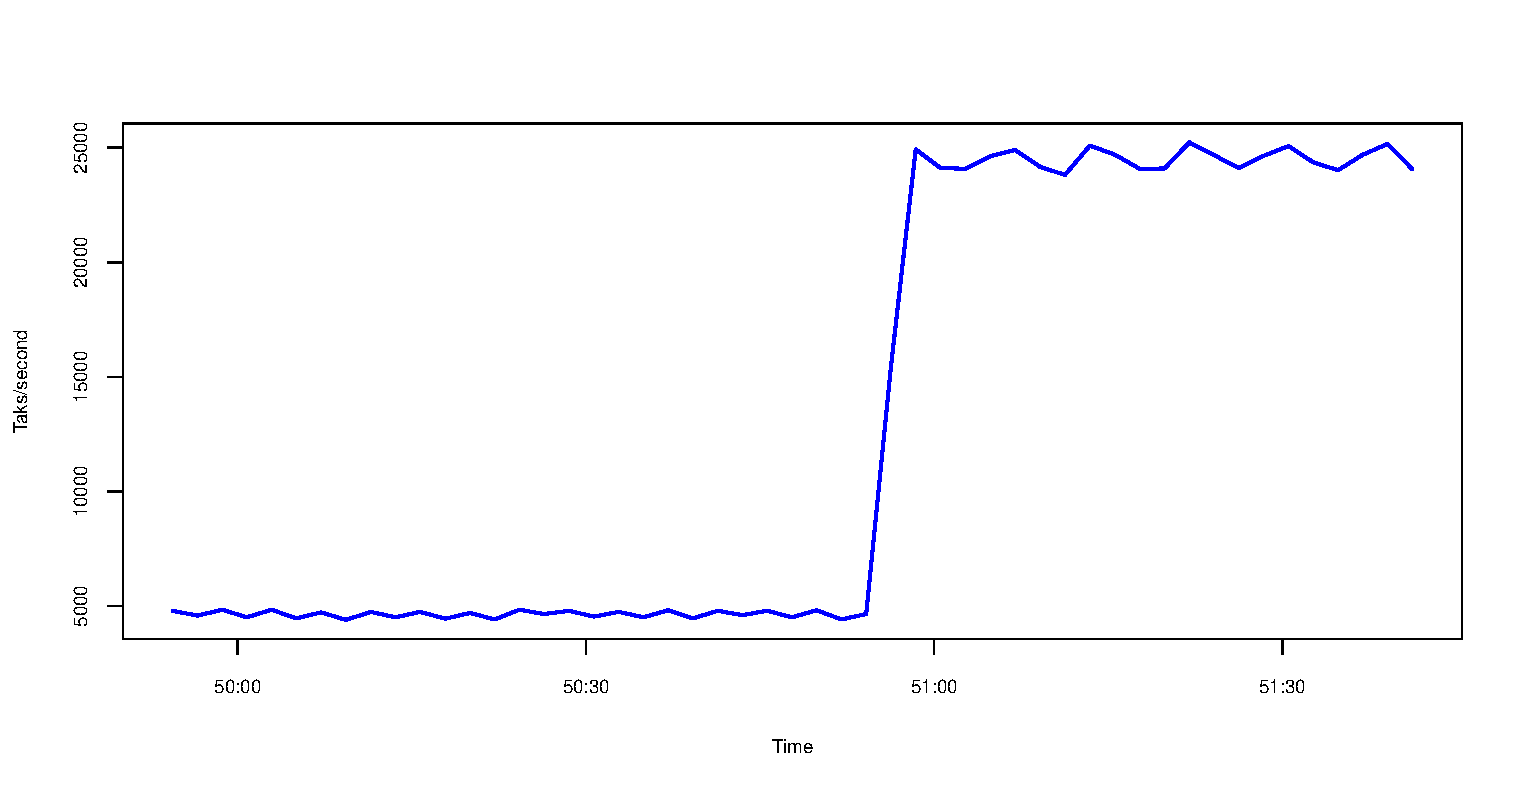
\includegraphics{stripchart}}}
\end{center}
\caption{Performance gain after adding workers to a running computation}
\end{figure}


Once the above example is running, the workers update the total number of tasks
taken in a Redis value called ``count'' at the start of each loop iteration. We
can use another R process to visualize a moving average of computational rate.
We ran the performance visualization R code in Listing \ref{perfvis}
on the ``master'' workstation after starting
the bootstrapping example (it requires the {\tt xts} time-series package).

We started the example bootstrap code running on the ``master'' system and the
logged in to the much more powerful Windows Server system and added four
additional workers using code in Listing \ref{addingworkers}. The resulting
performance plot clearly illustrates the dramatic increase in computational
rate when the new workers were added.

\subsection{A Parallel boot Function}

Listing \ref{bootforeach} presents a parallel capable variation of the {\tt
boot} function from the {\tt boot} package. The {\tt bootForEach} function uses
{\tt foreach} to distributed bootstrap processing to available workers. It has
two more arguments than the standard {\tt boot} function: {\tt chunks} and {\tt
verbose}. Set {\tt verbose=TRUE} to enabled back end worker process debugging.
The bootstrap resampling replicates will be divided into {\tt chunks} tasks for
processing by {\tt foreach}.  The example also illustrates the use of a custom
combine function in the {\tt foreach} loop.

\begin{lstlisting}[float=!ht,caption=Parallel boot Function,basicstyle=\footnotesize\ttfamily,label=bootforeach]
> bootForEach <- function (data, statistic, R, sim="ordinary",
>                  stype="i", strata=rep(1, n), L=NULL, m=0,
>                  weights=NULL, ran.gen=function(d, p) d,
>                  mle=NULL, simple=FALSE, chunks=1,
>                  verbose=FALSE, ...)
> {
>   thisCall <- match.call()
>   n <- if (length(dim(data)) == 2) nrow(data)
>   else length(data)
>   if(R<2) stop("R must be greater than 1")
>   Rm1 <- R - 1
>   RB <- floor(Rm1/chunks)

>   combo <- function(...)
>   {
>     al <- list(...)
>     out <- al[[1]]
>     t <- lapply(al, "[[", "t")
>     out$t <- do.call("rbind", t)
>     out$R <- R
>     out$call <- thisCall
>     class(out) <- "boot"
>     out
>   }
  
# We define an initial bootstrap replicate locally. We use this
# to set up all the components of the bootstrap output object
# that don't vary from run to run. This is more efficient for
# large data sets than letting the workers return this information.
>   binit <- boot(data, statistic, 1, sim = sim, stype = stype, 
>                 strata = strata, L = L, m = m, weights = weights,
>                 ran.gen = ran.gen, mle=mle, ...)
  
>   foreach(j=icount(chunks), .inorder=FALSE, .combine=combo,
+           .init=binit, .packages=c("boot","foreach"),
+           .multicombine=TRUE, .verbose=verbose)  %dopar% {
>    if(j==chunks) RB <- RB + Rm1 %% chunks
>    res <- boot(data, statistic, RB, sim = sim, stype = stype,
>                strata = strata, L = L, m = m, weights = weights,
>                ran.gen = ran.gen, mle=mle, ...)
>    list(t=res$t)
>  }
> }
\end{lstlisting}


\section{Technical Details}

A \verb+doRedis+ \emph{task} is a parameterized R expression that represents
a unit of work. The task expression is the body of a \verb+foreach+ loop. A
single task may consist of one or more loop iterations depending on the value
of the \verb+chunkSize+ parameter (the default is one).

All of the tasks associated with a single \verb+foreach+ statement are
collected into a \verb+doRedis+ \emph{job}. Each job is assigned a unique
identifier, and each job's tasks are enumerated $1, 2, 3, ...$.

Jobs are announced on a \emph{work queue}--technically, a special Redis key
called a ``list'' that supports blocking reads. Users choose the name of the
work queue in the \verb+registerDoRedis+ function. Master R programs that issue
jobs wait for results on yet another blocking Redis list, a result queue
specific to the job.

R workers listen on work queues for jobs using blocking reads.  As shown in the
last section the number of workers is dynamic.  It's possible for workers to
listen on queues before any jobs exist, or for masters to issue jobs to queues
without any workers available.


\subsection{Redis Key Organization}

The ``work queue'' name specified in the {\tt registerDoRedis} and
{\tt redisWorker} functions is used as the root name for a family of Redis
keys used to organize computation. Figure 2 illustrates example Redis
keys used by a master and worker R processes for a work queue named ``myjobs'',
described in detail below.

\begin{figure}[!ht]
\begin{center}
\resizebox{0.65\textwidth}{!}{\rotatebox{0}{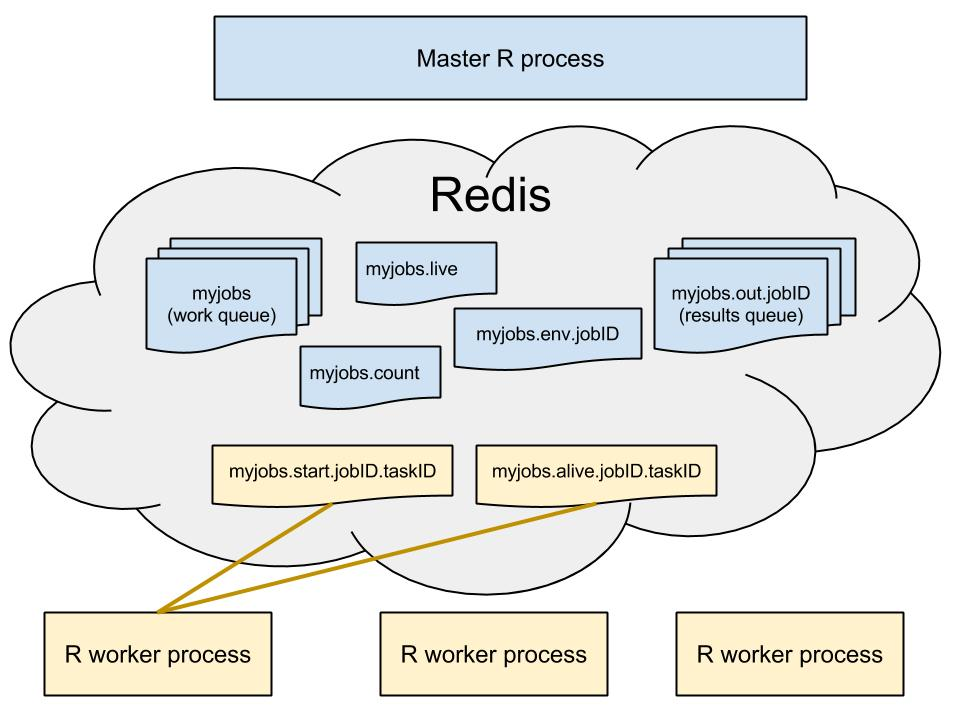
\includegraphics{keys}}}
\end{center}
\caption{Example {\tt doRedis} keys for an example work queue named ``myjobs''}
\label{keys}
\end{figure}

The name of the work queue illustrated in Figure 2 is ``myjobs.'' The
corresponding Redis key is also named ``myjobs'' and it's a Redis list value type
(that is, a queue).  Such a queue can be set up, for example, with
\verb+registerDoRedis(queue="jobs")+.

Removal of the ``jobs'' key serves as a signal that the work queue has been
removed, for example with the \verb+removeQueue("jobs")+ function. After this
happens, any R workers listening on the queue will clean up any Redis keys that
they created and terminate after a timeout period.

Along with the work queue, a counter key named ``myjobs.count'' is set up to
enumerate jobs. The key is atomically incremented by Redis with each new job.
It is an estimate of the number of workers currently registered to accept work
on the queue.

\verb+foreach+ assigns every job an R environment with state required to
execute the loop expression. The example in Figure 2 illustrates a job
environment for the ``myjobs'' queue and a particular job ID called
``jobs.env.jobID'' R worker processes working on ``jobID'' the ``myjobs'' queue
will download this environment key once (independently of the number of tasks
they run for the job).

All of the tasks for the job number 1 in the ``jobs'' queue are placed in a
Redis key called ``jobs:1`` in Figure 2. The Redis value type associated with
this key is a hash table. Hash table entries are named by task number ($1, 2,
...$) and the hash table values contain the \verb+foreach+ loop parameters
associated with the task.

The \verb+foreach+ loop performs the following steps to create a new job
in the ``jobs'' queue consisting of $n$ tasks:
\begin{enumerate}
\item Increment ``jobs:count'', recording the new job number
       (say, job number 1 for example).
\item Create and upload the  ``jobs:1.env'' job environment.
\item Populate the $n$ tasks in the ``jobs:1'' hash table with the
      \verb+foreach+ loop parameters for each task.
\item Push $n$ copies of the job number to the ``jobs'' queue to announce
  the new job with $n$ tasks.
\end{enumerate}

R workers listen on the ``jobs'' queue for new jobs. It's a blocking queue, but
the workers periodically time out. After each time out they check to see if the
``jobs:counter'' key still exists, and if it doesn't they terminate. If it's
still there, they loop and listen again for jobs.

When a job announcement arrives, a worker downloads the new job number
from the ``jobs'' queue. The worker then:
\begin{enumerate}
\item Checks the job number to see if it already has the job environment.
If it doesn't it downloads it (from ``jobs:1.env'' in the example).
\item Calls the \verb+getTask+ function defined in the job environment to
get a task. By default, this function pulls tasks in order from the
associated job task hash table (``jobs:1'' in Figure 2). The function
can be customized to do more (see the advanced examples topic in the sequel).
\item Upon successfully downloading a task, Redis
creates a task start key that indicates that the task is being processed.
The example in Figure 2 illustrates a task key called ``jobs:1.start.5''
indicating task number 5 of job number 1 in the jobs queue.
\item The R worker process maintains a task liveness key, illustrated
in Figure 2 as ``jobs:1.alive.5''.
\item When a task completes, the worker places the result in the job
result queue, shown in Figure 2 as ``jobs:1.results'', and then
removes its corresponding start and alive keys.
\end{enumerate}

Meanwhile, the R master process is listening for results on the job result
queue, shown in Figure 2 as ``jobs.1.results.'' Results arrive from the workers
as R lists of the form \verb+list(id=result)+, where \verb+id+ corresponds to
the task ID number and \verb+result+ to the computed task result.


\subsection{Worker Fault Detection and Recovery}

While running, each task is associated with two keys described in the last
section: a task ``started'' key and a task ``alive'' key. The ``started'' key
is normally created by Redis when a task is downloaded. The ``alive'' key is a
Redis ephemeral key with a relatively short time out (after which it
disappears). The R worker processes maintain background threads that keep the
ephemeral ``alive'' key active while the job is being run. If for some reason
the R worker process crashes, or the work system crashes or reboots, or network
fails, then the ``alive'' key will time out and be removed from Redis.

After \verb+foreach+ sets up a job, the master R process listens for results on
the associated job results queue. It's a blocking read, but the master R
process periodically times out. After each time out, the master examines all
the ``started'' and ``alive'' keys associated with the job. If it finds a
mismatch, the master R process assumes that task has failed and:
\begin{enumerate}
\item resubmits the task in the corresponding job tasks hash table;
\item announces another task for this job in the job queue.
\end{enumerate}

It's possible that a wayward R worker process might return after its task has
been declared lost. In such cases, results for tasks might be returned more
than once in the result queue, but \verb+doRedis+ is prepared for this and
simply discards repeated results.


\subsection{Random Number Generator Seeds}

The initialization of pseudorandom number generators is an important
consideration, especially when running simulations in parallel. Each {\tt
foreach} loop iteration (task) is assigned a number in order from the sequence
$1, 2, \ldots$. By default, {\tt doRedis} workers initialize the seed of their
random number generator with a multiple  of the first task number they receive.
The multiple is chosen to very widely separate seed initialization values.
This simple scheme is sufficient for many problems, and comparable to
the initialization scheme used by many other parallel back ends.

\begin{lstlisting}[float=!ht,caption=User-defined RNG initialization,label=rng]
# First, use the default initialization:
> startLocalWorkers(n=5,queue="jobs")
> registerDoRedis("jobs")
> foreach(j=1:5,.combine="c") %dopar% runif(1)
 [1] 0.27572951 0.62581389 0.90845008 0.49669130 0.06106442 

# Now, let's make all the workers use the same random seed initialization:

> set.seed.worker <- function(n) set.seed(55)
> foreach(j=1:5,.combine="c",.export="set.seed.worker") %dopar% runif(1)
[1] 0.5478135 0.5478135 0.5478135 0.5478135 0.5478135
\end{lstlisting}

The {\tt doRedis} package includes a mechanism to define an arbitrary random
seed initialization function. Such a function could be used, for example, with
the {\tt SPRNG} library or with the \verb+doRNG+ package for \verb+foreach+.

The user-defined random seed initialization function must be called {\tt
set.seed.worker}, take one argument and must be exported to the workers
explicitly in the {\tt foreach} loop. The example shown in Listing \ref{rng}
illustrates a simple user-defined seed function.


\subsection{Known Problems and Limitations}

If CTRL+C is pressed while a {\tt foreach} loop is running, connection to the
Redis server may be lost or enter an undefined state. An R session can reset
connection to a Redis server at any time by issuing \verb+redisClose()+
followed by re-registering the {\tt doRedis} back end.

Redis limits database values to less than 2\,GB. Neither the \verb+foreach+
loop parameters nor the job environment may exceed this size. If you need to
work on chunks of data larger than this, see the Advanced Topics section
for examples of working on already distributed data in place.




\section{Advanced Topics}

Let's start this section by dealing with the 2\,GB Redis value size limit.
Problems will come along in which you'll need to get more than
2\,GB of data to the R worker processes. There
are several approaches that one might take:
\begin{enumerate}
\item Distribute the data outside of Redis, for example through a shared
      distributed file system like PVFS or Lustre.
\item Break the data up into chunks that each fit into Redis and use
      Redis to distribute the data.
\end{enumerate}
The first approach is often a good one, but is outside of the scope of this
vignette. We illustrate the second approach in the following example.
For the purposes of illustration, the example matrix is tiny and we break it
up into only two chunks. But the idea extends directly to very large
problems.

\begin{lstlisting}[float=!ht,caption=Explicitly breaking a problem up into chunks,basicstyle=\footnotesize\ttfamily,label=chunk]
> registerDoRedis("jobs")

> set.seed(1)
> A <- matrix(rnorm(100),nrow=10)   # (Imagine that A is really big.)

# Partition the matrix into parts small enough to fit into Redis values
# (less than 2GB). We partition our example matrix into two parts:

> A1 <- A[1:5,]      # First five rows
> A2 <- A[6:10,]     # Last five rows

# Let's explicitly assign these sub-matrices as Redis values. Manually breaking
# up the data like this helps avoid putting too much data in the R environment
# exported by foreach.

> redisSet("A1", A1)
> redisSet("A2", A2)

> ans <- foreach(j=1:2, .combine=c) %dopar% {
>   chunk <- sprintf("A%d",j)
>   mychunk <- redisGet(chunk)
>   sum(mychunk)
> }

> print(ans)
[1] 6.216482 4.672254
\end{lstlisting}

The point of the example in Listing \ref{chunk} is that the workers explicitly
download just their portion of the data inside the \verb+foreach+ loop. This
avoids putting the data into the exported R environment, which could exceed the
Redis 2\,GB value size limit. The example also avoids sending data to workers
that they don't need. Each worker downloads just the data it needs and nothing
more.


\subsection{Custom task assignment}

The example shown in Listing \ref{chunk} presents one way to distribute just
the data needed to each task. But what if we need to repeat the \verb+foreach+
loop in Listing \ref{chunk}, for example in the running of an iterative method?
It would be nice if the workers could cache their chunks of data locally and
simply re-use that without fetching new data.

The default \verb+doRedis+ approach assigns work to workers on a first-come,
first-served basis. But it also allows for custom task assignment, for example
to align tasks with existing cached data on workers. Custom task assignment can
also be used to allocate tasks based on distance to already distributed data.


Let's recall how tasks are assigned to a worker R process by \verb+doRedis+
(refer to Figure \ref{keys}):
\begin{enumerate}
\item The worker waits for a job announcement with a blocking
      read on the job work queue (``jobs'' in Figure \ref{keys}).
\item After a job ID is removed from the work queue, the worker
      downloads the job R environment value (``jobs:1.env'').
\item The environment contains a function called \verb+getTask+. The
      worker invokes this function with the work queue name, the job ID,
      and a worker ``tag'' value to get a task.
\item If a task was obtained, the worker executes it, placing the result
      in the result queue \break(``jobs.1.results''). Otherwise the worker
      replaces the obtained job ID into the work queue and repeats
      (see below for a discussion of this exceptional case).
\end{enumerate}
Customization of task assignment boils down to supplying a custom
\verb+getTask+ and setting a ``tag'' value in the workers.


\subsubsection{Setting worker tags}

A ``tag'' is a character string that workers report to their \verb+getTask+
functions. Tags can be any character string, and they do not need to be unique.
Workers report their system host names by default. Interesting tag possibilities
are chunk number and worker I.P. address.

Set tags with the \verb+setTag+ function. This step is usually done once in the
first \verb+foreach+ loop.  Once a tag is set, it remains in force until reset
(the tag value will not vary from job to job).


\subsubsection{Customizing the getTask function}

The task assignment decision is made by the Redis server.  The default
\verb+getTask+ function specifies a Lua script that is run by Redis. It
ignores the ``tag'' argument supplied by the workers.  Here it is:
\begin{lstlisting}[float=!ht,caption=Default getTask function,basicstyle=\footnotesize\ttfamily,label=getTask]
getTask <- function(queue, job_id, ...)
{
  key <- sprintf("
  redisEval("local x=redis.call('hkeys',KEYS[1])[1];
             if x==nil then return nil end;
             local ans=redis.call('hget',KEYS[1],x);
             redis.call('set', KEYS[1] .. '.start.' .. x, x);
             redis.call('hdel',KEYS[1],x);i
             return ans",key)
}
\end{lstlisting}
Note that it's important for the \verb+getTask+ function to set the task started
key (the Lua statement \verb+redis.call('set', KEYS[1] .. '.start.' .. x, x)+).
For reliable operation, this should be set by Redis and not left up to the
R worker.

Let's modify the example in Listing \ref{chunk} to preferentially assign work
to workers that already have locally cached data.  With these modifications in
place, the \verb+foreach+ loop in Listing \ref{chunk} can be repeated without
incurring any new data movement costs as long as the \verb+doRedis+ worker pool
remains constant.

\begin{lstlisting}[float=!ht,caption=Custom getTask function,basicstyle=\footnotesize\ttfamily,label=custom]
> myGetTask <- function(queue, job_id, tag, ...)
{ 
# The default task Redis hash map is labeled queue:job_id:
>   key <- sprintf("%s:%s",queue, job_id)
# The worker tag is passed in to the Redis Lua interpreter as ARGV[1].
# See ?redisEval for details.
>   redisEval("local x=redis.call('hkeys',KEYS[1])[tonumber(ARGV[1])];
+              if x==nil then x=redis.call('hkeys',KEYS[1])[1]; end;
+              if x==nil then return nil; end;
+              local ans=redis.call('hget',KEYS[1],x);
+              redis.call('set', KEYS[1] .. '.start.' .. x, x);
+              redis.call('hdel',KEYS[1],x);
+              return ans",key,FALSE,tag)
}
\end{lstlisting}

The custom \verb+myGetTask+ function shown in Listing \ref{custom} first tries
to assign a specific task number requested by the worker via its tag. If that
fails, it assigns the first available task or NULL if there aren't any tasks.
Listing \ref{customloop} shows a modified version of the \verb+foreach+ loop
from example \ref{chunk}. The modifications add the following:
\begin{mitemize}
\item Cache the data in the worker's R global environment the first time run.
\item Assign a tag corresponding to the cached data chunk.
\item Use the custom \verb+myGetTask+ function from Listing \ref{custom}.
\item Add some debugging output to help understand what's happening.
\end{mitemize}

\begin{lstlisting}[float=!ht,caption=Modified foreach loop,basicstyle=\footnotesize\ttfamily,label=customloop]
> ans  <-
> foreach(j=1:2, .options.redis=list(getTask=myGetTask)) %dopar% {
>   chunk <- sprintf("A%d",j)
>   log <- paste("My job is to sum chunk ",chunk)
>   log <- paste(log,"My tag ID is ",doRedis:::.getTag())
# Check if we have a cached copy of the chunk
>   if(exists(chunk))
>   {
>     log <- paste(log,"I've already got this chunk...")
>     mychunk <- get(chunk)
>     return(list(sum=sum(mychunk), log=log))
>   }
# We don't have it cached, download it and cache it locally...
>   log <- paste(log,"Downloading chunk",chunk)
>   setTag(j)     # Set our tag!
>   assign(chunk, redisGet(chunk), envir=globalenv())
>   mychunk <- get(chunk, envir=globalenv())
>   list(sum=sum(mychunk), log=log)
> }
> print(ans)
\end{lstlisting}

Let's say that the example shown in Listing \ref{customloop} is run
using the ``jobs'' work queue with two local \verb+doRedis+ workers,
for example with:
\begin{lstlisting}[float=!ht,caption=Starting two local R workers,xleftmargin=0pt]
> library("doRedis")
> registerDoRedis("jobs")
> startLocalWorkers(n=2, queue="jobs")
\end{lstlisting}
The first time you run the example \verb+foreach+ loop in Listing
\ref{customloop}, you'll see output similar to that shown
in Listing \ref{exampleoutput1} below.
\begin{lstlisting}[float=!ht,caption=First foreach loop run,label=exampleoutput1]
[[1]]
[[1]]$sum
[1] 0
  
[[1]]$log
[1] "My job is to sum chunk  A1 My tag ID is localhost Downloading chunk A1"
  
  
[[2]]
[[2]]$sum
[1] 0
  
[[2]]$log
[1] "My job is to sum chunk  A2 My tag ID is localhost Downloading chunk A2"
\end{lstlisting}
If you repeat the \verb+foreach+ loop in Listing \ref{customloop}, you'll see output
similar to that shown below in Listing \ref{exampleoutput2}, which shows that the
workers are using their cached data. You can repeat the \verb+foreach+ loop as many
times as you like and the output should remain constant.
\begin{lstlisting}[float=!ht,caption=Repeated foreach loop runs,label=exampleoutput2]
[[1]]
[[1]]$sum
[1] 0

[[1]]$log
[1] "My job is to sum chunk  A1 My tag ID is  1 I've already got this chunk..."


[[2]]
[[2]]$sum
[1] 0

[[2]]$log
[1] "My job is to sum chunk  A2 My tag ID is  2 I've already got this chunk..."
\end{lstlisting}

Note that, even if one of the workers quits or crashes, the remaining worker
will be assigned work to finish the job. And, the method still accommodates
additional workers coming on line at any time.


\subsection{Things to watch out for}

\verb+foreach+ submits all tasks associated with one job in a single Redis
transaction. This is important in light of the custom task pulling example in
Listing \ref{custom}.  We'd like to make sure that all the tasks are available
before doling out work to avoid prematurely assigning a task to the wrong
worker.

However, that means that if the \verb+foreach+ loop parameterization contains a
lot of data, there can be a significant lag before starting the work. Avoid
loop parameterizations containing lots of data. It's a better idea to manually
break up data into Redis keys as shown in the example in Listing \ref{chunk}.

It's possible that a worker can remove a job announcement from a work queue
without requesting a task via \verb+getTask+ from the job's task set. That's
a problem. Another problem already discussed in the fault tolerance section
occurs when the number of started tasks does not match the number of alive
tasks.  The master process periodically checks two things:
\begin{enumerate}
\item Number of started tasks = number of alive tasks (fault check)
\item queued + started + finished = total
\end{enumerate}
If item 2 fails, then the queue is out of balance and the master R program
resubmits the missing number of task entries. In either case, it's possible
that a rogue worker process tricks us and completes work that apparently
failed. The master R program running the \verb+foreach+ loop throws away
replicated task results, keeping only the first result to arrive.


\subsection{worker.init}

If you export a function named \verb+worker.init+ that takes no arguments, it
will be run by the workers once just after downloading a new job environment.
This is a generic function that may contain any worker initialization code that
may not be appropriate for the body of the \verb+foreach+ loop.
The \verb+worker.init+ function is rarely needed.

\end{document}
